\documentclass[a4paper,12pt]{article}
\usepackage[notoc,noabs]{HaotianReport}

\title{基于文本数据挖掘的官媒主题效力分析}
\author{刘昊天}
\authorinfo{lht18@mails.tsinghua.edu.cn}
\runninghead{清华大学《政务大数据》2019秋季学期}
\studytime{2019年12月}

\begin{document}
    \maketitle
    \section{研究背景}
    所谓“官媒”,通常指的是有政府背景,由政府部门创办的媒体。它具有专用、权威、公开等性质,是官方监督与纠正不良现象、协调社会关系、传承文化、提供娱乐、引导大众、传播资讯的重要渠道\cite{guanmei}。一直以来,官媒都有其独有的优势,包括公信力优势、资金政策优势、人才优势和融媒体优势\cite{李志明2017区域性官媒和自媒体微信公众号差异化分析}。如何更好地发挥官媒优势,增强官媒的影响力与传播力,进而更充分地完成官方赋予官媒的使命,是官方机构工作人员长期以来关注的问题。

    传统的官媒形式包括报纸、电台、电视等,在新中国建设中发挥过重要作用。然而,随着网络时代的到来,智能手机不断普及,移动社交软件已经渐渐成为人们生活的重要组成部分,媒介形式也迎来了翻天覆地的变化。最有代表性的微信,作为目前腾讯旗下赶超 QQ 的社交软件,更是在前几年迎来爆发式增长。根据腾讯控股 [00700]2018年年报,截止至 2018 年 12 月 31,微信合并月活跃用户数达 10.98 亿,同比增长 11.0\%;同时, 2018 年腾讯的网络广告业务收入达 581 亿元,同比增长 44\%。

    在微信及腾讯广告业务的发展过程中,微信公众号功不可没,其已经成为了国内最大的内容提供平台之一,也从一种社交新宠逐渐演变成民间自媒体的一种主要形式并几近泛滥。个人或企业用户可以在微信公众号上发布文章,通过微信的订阅服务定向推送给已订阅的用户,无论是宣传还是营收都有巨大的空间;已订阅用户则可以消费微信公众号的推送内容。数据显示,2013年至2017年,微信公众号数量增长近10倍,如\cref{fig:pub}所示。
    由此可见,微信公众号已经并将在很长一段时间内继续扮演中国人生活中的重要角色。

    \begin{figure}
      \centering
      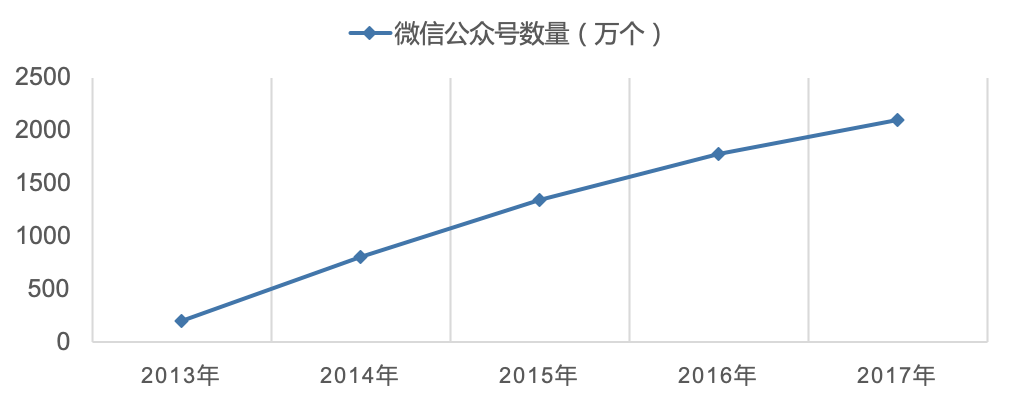
\includegraphics[width=0.9\linewidth]{pub.png}
      \caption{微信公众号数量统计}
      \label{fig:pub}
    \end{figure}

    为顺应该形势,近年来各地政府纷纷开通微信公众号作为官媒的新形式,发挥着宣传渠道、服务平台与展示窗口的关键作用。由此,本文拟采用官方或官方媒体的微信公众号作为官媒的代表进行研究。

    \section{研究问题}
    尽管官媒发布的内容往往是经由工作团队精心挑选或编写的,但受众并非对于官媒发布的所有内容都感到兴趣。换言之,即便在相同的官媒中,发布不同的官媒内容也将呈现出不同的传播效力。

    以目前微信平台上目前最大的官方媒体之一“人民日报”为例,2019年8月19日发布的题为《为了一名高三女孩,末班公交每天多等5分钟,直到她考上大学……》一文,收获了10万以上阅读量,10万以上点赞量;而在2019年8月26日发布的题为《【提醒】微信工作群“说错话”,被公司状告赔偿46万》一文,尽管同样收获了10万以上阅读量,却只有767点赞量。
    
    再以吉林省的官方媒体之一“吉林日报”为例,其平均阅读量和点赞量都远不及“人民日报”。2019年10月9日发布的题为《定了!吉林省这些院校和专业成为省级示范,有你的母校吗?》一文,收获了90906阅读量和302点赞量;而在2019年11月15日发布的题为《动车票低至6.5折、敞开办理团体票业务…吉林车务段推出超多优惠!》一文,却仅收获了670阅读量和3点赞量。
    
    由此两例可见,官媒发布的文本内容同传播效力之间存在一定的联系。本文的目标即为刻画官媒文本内容同该内容传播效力之间的关系(简称“内容-效力关系”),为官媒内容发布提供参考。特别地,选取文本内容的主题作为核心特征,因其一方面易于被人们解读,另一方面也能将文本数据转换为数值数据,便于分析。本文的到的相关结构,可以指导官媒在媒介资源有限的条件下最大化传播效力,充分发挥官媒功能。

    另外,本文也希望通过对比官媒与非官媒、不同官媒之间的内容-效力关系,分析各个公众号的内容特质。
    \section{研究方法}
    
    \subsection{主题提取}
    在对大量的公众号文章进行文本挖掘时, 一个自然的想法是利用一系列可以概括文章内容的主题来对文本库进行分析归纳。本文采用的主题模型一方面将大量繁杂的文章映射到一组低维度主题词上,另一方面,不同于简单的文本聚类模型,聚类后每篇文章仅能属于一个主题类别,主题模型可以在对文章进行分类整合的同时,允许不同文章间内容和立意的重叠,并能量化地表现出主题的相似度。

    在实际进行主题提取时, 本文采用文本挖掘领域最常用且有效的主题模型算法LDA(Latent Dirichlet Allocation), 这一算法基于对文本建立主题模型过程中所遵循的两个核心原则:
    
    \begin{itemize}
      \item \textbf{每篇文章是一系列主题的组合}:每篇文章包含了以一定比例混合的主题。比如, 文档一包含$10\%$的A主题和$90\%$的B主题; 文档二包含了$80\%$的A主题和$20\%$的B主题;
      \item \textbf{每个主题是一系列词语的组合}:主题的产生源于以一定比例混合的词语。比如
      娱乐主题中包含“电影”“电视”等词;政治主题中则更多包含“环境”、“民生”等词。值得注意的是,每个主题下所包含的关键词及其配比并非通过先验知识人为给定,而是在整个大的文本数据库中,利用无监督的机器学习算法提取而出。
    \end{itemize}
    
    \subsection{多元回归分析}
    多元回归分析主要用于分析响应变量与一系列解释变量之间的线性相关性和依赖性,以此来进行统计解释、推断和预测。记$Y$为我们所关心的响应变量,$V_1,...,V_K$为解释变量,回归分析所基于的多元线性模型为:
    \begin{equation}\label{lm}
      Y = \beta_0+ \beta_1 V_1+...+\beta_K V_K +\epsilon,
    \end{equation}
    这里$\epsilon \sim N(0,\sigma^2)$ 为模型中引入的同方差独立高斯噪声。
    
    利用最小二乘法,我们可以得到对线性模型参数的估计量$\hat\beta_0,...,\hat\beta_K$以及其他相关回归统计量。根据模型(\ref{lm}),我们可以进行以下统计推断:
    \begin{itemize}
      \item 回归得到的改进的$R^2$系数和$F$统计量对应的p值可以用来衡量线性模型整体的显著性;
      \item 每个解释变量系数所对应的t统计量及其对应的p值可用于衡量该单一变量在模型中的显著性;
      \item 当解释变量线性无关且具有相同量纲时,多元回归得到的变量系数大小可以用来比较解释变量对响应变量的影响大小;而变量系数的符号则可用来衡量该解释变量对响应变量(文章效力)的作用方向。
    \end{itemize}
    \section{数据来源及变量测量}
    \subsection{数据来源}
    介绍爬取方式。
    简单的样本描述
    \subsection{效力分析}
    量化单篇推送的传播效力。
    \section{研究发现及结果解释}
    \begin{table}[!htbp] \centering 
      \caption{} 
      \label{} 
    \begin{tabular}{@{\extracolsep{5pt}} ccccc} 
    \\[-1.8ex]\hline 
    \hline \\[-1.8ex] 
     & Estimate & Std. Error & t value & Pr(\textgreater \textbar t\textbar ) \\ 
    \hline \\[-1.8ex] 
    V1 & $$-$0.369$ & $0.047$ & $$-$7.910$ & $0$ \\ 
    V2 & $0.182$ & $0.042$ & $4.277$ & $0.00002$ \\ 
    V3 & $$-$0.354$ & $0.034$ & $$-$10.448$ & $0$ \\ 
    V4 & $$-$0.233$ & $0.038$ & $$-$6.172$ & $0$ \\ 
    V5 & $0.012$ & $0.041$ & $0.300$ & $0.764$ \\ 
    V6 & $$-$0.251$ & $0.030$ & $$-$8.262$ & $0$ \\ 
    V7 & $0.318$ & $0.043$ & $7.421$ & $0$ \\ 
    V8 & $$-$0.214$ & $0.040$ & $$-$5.283$ & $0.00000$ \\ 
    V9 & $0.440$ & $0.061$ & $7.269$ & $0$ \\ 
    \hline \\[-1.8ex] 
    \end{tabular} 
    \end{table} 
      \begin{enumerate}
        \item 样本描述
        \begin{enumerate}
          \item 观测范围(时间、空间)
          \item 数据量
          \item 数据分布
          \item 公众号的分布
        \end{enumerate}
        \item 效力分析:如何量化单篇推送的传播效力
        \item 主题提取
        \item 情感分析
        \item 相关性分析 (主题 - 效力) (情感 - 效力)
      \end{enumerate}
    \label{applastpage}
    \newpage
    \bibliography{report}
    \bibliographystyle{unsrt}
\iffalse
\begin{itemize}[noitemsep,topsep=0pt]
%no white space
\end{itemize}
\begin{enumerate}[label=\Roman{*}.,noitemsep,topsep=0pt]
%use upper case roman
\end{enumerate}
\begin{multicols}{2}
%two columns
\end{multicols}
\begin{figure}
  \centering
  \includegraphics[width=0.9\linewidth]{}
  \caption{}
  \label{fig:}
\end{figure}
\fi
\end{document}
